\documentclass[11pt,a4paper]{article}
\usepackage[utf8]{inputenc}
\usepackage{amsmath,amssymb,amsfonts}
\usepackage{graphicx}
\usepackage{booktabs}
\usepackage{subcaption}
\usepackage{hyperref}
\usepackage{geometry}
\geometry{margin=2.4cm}
\graphicspath{{figures/}}

\title{Improving GBS-Based Sampling of Classical Distributions:\\
Matrix Construction, Encoding, Optimisation and Readout}
\author{I.B., L.E.C.E., V.V.P.}
\date{}

\begin{document}
\maketitle

\begin{abstract}
We study the use of Gaussian Boson Sampling (GBS) as a trainable generative
model for one-dimensional classical distributions discretised into bit strings.
Starting from the variational WAW framework, we identify and correct a chain of
distinct bottlenecks: a biased initial adjacency-matrix construction, a
representation-hostile bit-string encoding, an unreliable optimisation loop, an
uncontrolled photon-number budget, and the choice of detector (threshold vs
photon-counting). For each we give the physical motivation, the method, and the
measured effect on the Kullback--Leibler (KL) divergence between the learned and
target distributions. The combination of a per-pair/parity construction, a
Gray-code encoding, an analytic keep-best optimiser, and photon-number matching
reduces the KL by roughly a factor of three relative to the baseline on smooth
targets, and by about $2.5\times$ on a multimodal target. We further show that
the residual error on multimodal targets is an expressivity floor of a single
Gaussian state, that the detector choice should be matched to the target's
concentration, and that a persistent central spike is controlled by the mean
photon number rather than by any objective reweighting.
\end{abstract}

\tableofcontents

\section{Problem statement}

A GBS device with threshold detectors produces click patterns $s\in\{0,1\}^m$
whose probabilities are fixed by a symmetric adjacency matrix $A$ through the
torontonian. In the variational (WAW) approach of Banchi
\textit{et~al.}~\cite{banchi2020}, $A$ is first built from training samples and
then refined by trainable per-mode weights $W$, $A\mapsto WAW$, to minimise the
KL divergence to a target distribution. We take as target a smooth
one-dimensional density $p(x)$ discretised into $K=2^{m}-2$ bins (dropping the
all-zero and all-one patterns), and encode each bin as a click pattern.

This report documents a sequence of improvements to that pipeline. Quality is
measured by $D_{\mathrm{KL}}(p_{\mathrm{target}}\|p_{\mathrm{model}})$, evaluated
either from Monte-Carlo samples (early figures) or, where noted, exactly from
the analytic click distribution (tables). We use three smooth targets (normal,
log-normal) and a multimodal target, and later add sharp (Cauchy) and
asymmetric-bimodal targets.

\section{Background: the factorial/parity bias}

For a zero-mean Gaussian state the photon-number probability is
\begin{equation}
P(\mathbf{n})=\frac{1}{\sqrt{\det Q}}\,\frac{|\mathrm{Haf}(A[\mathbf{n}])|^{2}}
{\prod_i n_i!},
\end{equation}
where $A[\mathbf{n}]$ repeats row/column $i$ exactly $n_i$ times. The hafnian of
an odd-dimensional matrix vanishes, so any contributing configuration has an
even total photon number. A threshold detector reports only the support
$s_i=\mathbb{1}[n_i\ge 1]$, summing $P(\mathbf{n})$ over all configurations with
a given support. Two consequences drive the report: (i) every \emph{odd}-click
pattern must double one mode to reach an even photon count, incurring a $1/2!$
suppression absent for even-click patterns; (ii) the collision configurations
($n_i\ge 2$) that threshold detection folds into a click are exactly the
information a photon-counting detector would resolve.

\section{Methods}

\subsection{Initial construction}

\paragraph{Corrected construction.}
The original \texttt{A\_from\_samples} adds diagonal self-loops only for
single-click samples. \texttt{A\_from\_samples\_corrected} counts a self-loop
for every clicking mode and boosts the diagonal by $\sqrt{2}$ to compensate the
two-photon bunching term $P(n_i{=}2)\propto |A_{ii}|^2/2!$. This is motivated
only by the $k=1$ case.

\paragraph{Parity rule.}
The same $1/2!$ factor appears for \emph{every} odd-click pattern.
\texttt{A\_from\_samples\_parity} weights each sample by $w_s=\sqrt{2}$ if
$k=|s|$ is odd and $1$ if even, applied to all self-loops and edges it touches.
It reduces to the $\sqrt{2}$ boost for $k=1$ and additionally corrects edge
counts from odd-click samples.

\paragraph{Per-pattern weights.}
Summing over all photon configurations under a uniform reference $A_0=\alpha J$
gives closed-form per-$k$ weights $w_k=R(2)/R(k)$ with
$f_k(N)=[x^N](e^x-1)^k$ (\texttt{A\_from\_samples\_perpattern}). Empirically
this over-suppresses high-$k$ samples ($w_3\approx0.07$), discarding real
pair-correlation information, and was abandoned.

\paragraph{Per-pair normalisation.}
A $k$-click sample deposits into $\binom{k}{2}$ edges and $k$ loops, so high-$k$
samples flood the matrix. \texttt{A\_from\_samples\_perpair} divides each
sample's contribution by the number of entries it touches,
$A_{ii}\mathrel{+}=w_s/k$, $A_{ij}\mathrel{+}=w_s/\binom{k}{2}$, keeping the
parity weight. It is the most robust construction.

\paragraph{Photon-number (variance) matching.}
Rescaling fixes only the mean photon number; the variance of the click count
$k$ is uncontrolled. \texttt{A\_from\_samples\_variance} matches the full
click-count histogram $h(k)$ by iterative proportional fitting,
$\rho_k \leftarrow \rho_k\,[\,h_{\mathrm{data}}(k)/h_{\mathrm{model}}(k)\,]^{\alpha}$
(clipped), with a tunable prefactor $\alpha$.

\subsection{Encoding}
The default encoding uses the \emph{standard binary} representation of the bin
index, which is not Hamming-smooth: adjacent bins can differ in all $m$ bits.
A reflected Gray code $g(n)=n\oplus(n\gg1)$ (\texttt{gray\_encoding}) makes
consecutive bins differ in one bit, keeping a smooth target piecewise-smooth in
pattern space. \texttt{rank\_assign} additionally chooses a probability-matched
encoding (largest target mass on the most-probable outcome), and
\texttt{empirical\_target\_from\_data} estimates the target shape from samples
alone so the encoding is realizable without knowing the target.

\subsection{Optimisation}
The baseline WAW uses random initialisation and returns the last iterate; on
Gray-encoded data it collapsed onto one mode. \texttt{train\_WAW\_bestkl} uses
zero initialisation and keep-best return. Crucially,
\texttt{torontonian\_sample\_graph} silently rescales $A$ at sampling time, so
the optimised and evaluated distributions differed and the reported KL could
\emph{increase} after training; \texttt{train\_WAW\_analytic} removes this by
minimising the exact analytic KL (loop torontonian over all $2^m$ patterns) with
keep-best return, so KL never increases.

\subsection{Displacement}
Squeezed vacuum contains only even photon numbers, biasing click parity.
\texttt{train\_displaced\_gbs} trains the full displacement
$\boldsymbol\mu\in\mathbb{R}^{2m}$ (small $m$ only);
\texttt{train\_waw\_then\_displace} is a scalable surrogate (WAW then a single
scalar displacement tuned by binary search to match the odd-parity fraction);
\texttt{train\_parity\_mixing} is a classical two-circuit workaround.

\subsection{Readout}
A counting detector reads $\mathbf{n}$ directly; for a collision-free pattern
$P(\mathbf{n})\propto|\mathrm{Haf}(A_S)|^2$ over the support submatrix
(\texttt{pnr\_readout}). \texttt{train\_threshold\_nmean} exposes the mean photon
number $n_{\mathrm{mean}}$ as a tunable, used below to control concentration;
\texttt{select\_nmean} picks it by minimising the empirical KL, and
\texttt{combine\_threshold\_pnr} forms the empirical-best convex mixture of the
two readouts.

\section{Results}

\subsection{Initial construction and encoding}
Table~\ref{tab:constr} reports the analytic KL after WAW for every construction,
target and encoding at $m=5$ (2000 samples). Three conclusions stand out. The
construction refinements dominate for the smooth targets (normal, log-normal),
cutting the baseline KL by roughly $2$--$3\times$. The Gray encoding is decisive
for the multimodal target, more than halving its KL
($0.59\to0.24$). The variance construction is best or tied-best on the smooth
and multimodal targets, and per-pair on the log-normal.

\begin{table}[h]
\centering
\begin{tabular}{lcccccc}
\toprule
 & \multicolumn{2}{c}{Normal} & \multicolumn{2}{c}{Multimodal} & \multicolumn{2}{c}{Log-normal}\\
\cmidrule(lr){2-3}\cmidrule(lr){4-5}\cmidrule(lr){6-7}
Construction & binary & Gray & binary & Gray & binary & Gray\\
\midrule
Baseline              & 0.56 & 0.57 & 0.61 & 0.38 & 0.61 & 0.63\\
Parity                & 0.21 & 0.13 & 0.59 & 0.24 & 0.34 & \textbf{0.24}\\
Per-pair              & 0.20 & 0.14 & 0.59 & 0.28 & 0.30 & 0.25\\
Variance ($\alpha{=}0.5$) & 0.19 & \textbf{0.13} & 0.58 & \textbf{0.27} & 0.33 & 0.25\\
\bottomrule
\end{tabular}
\caption{Analytic KL after WAW ($m=5$). Best per target/encoding in bold; the
best absolute values are $0.13$ (normal, variance+Gray), $0.24$ (multimodal,
parity+Gray) and $0.24$ (log-normal, parity+Gray).}
\label{tab:constr}
\end{table}

Figure~\ref{fig:fix} shows the per-pair construction against the baseline and
per-pattern for the multimodal and log-normal targets: it removes the high-click
overshoot of the baseline and the low-click overshoot of the per-pattern
weights.

\begin{figure}[h]
\centering
\begin{subfigure}{0.49\textwidth}
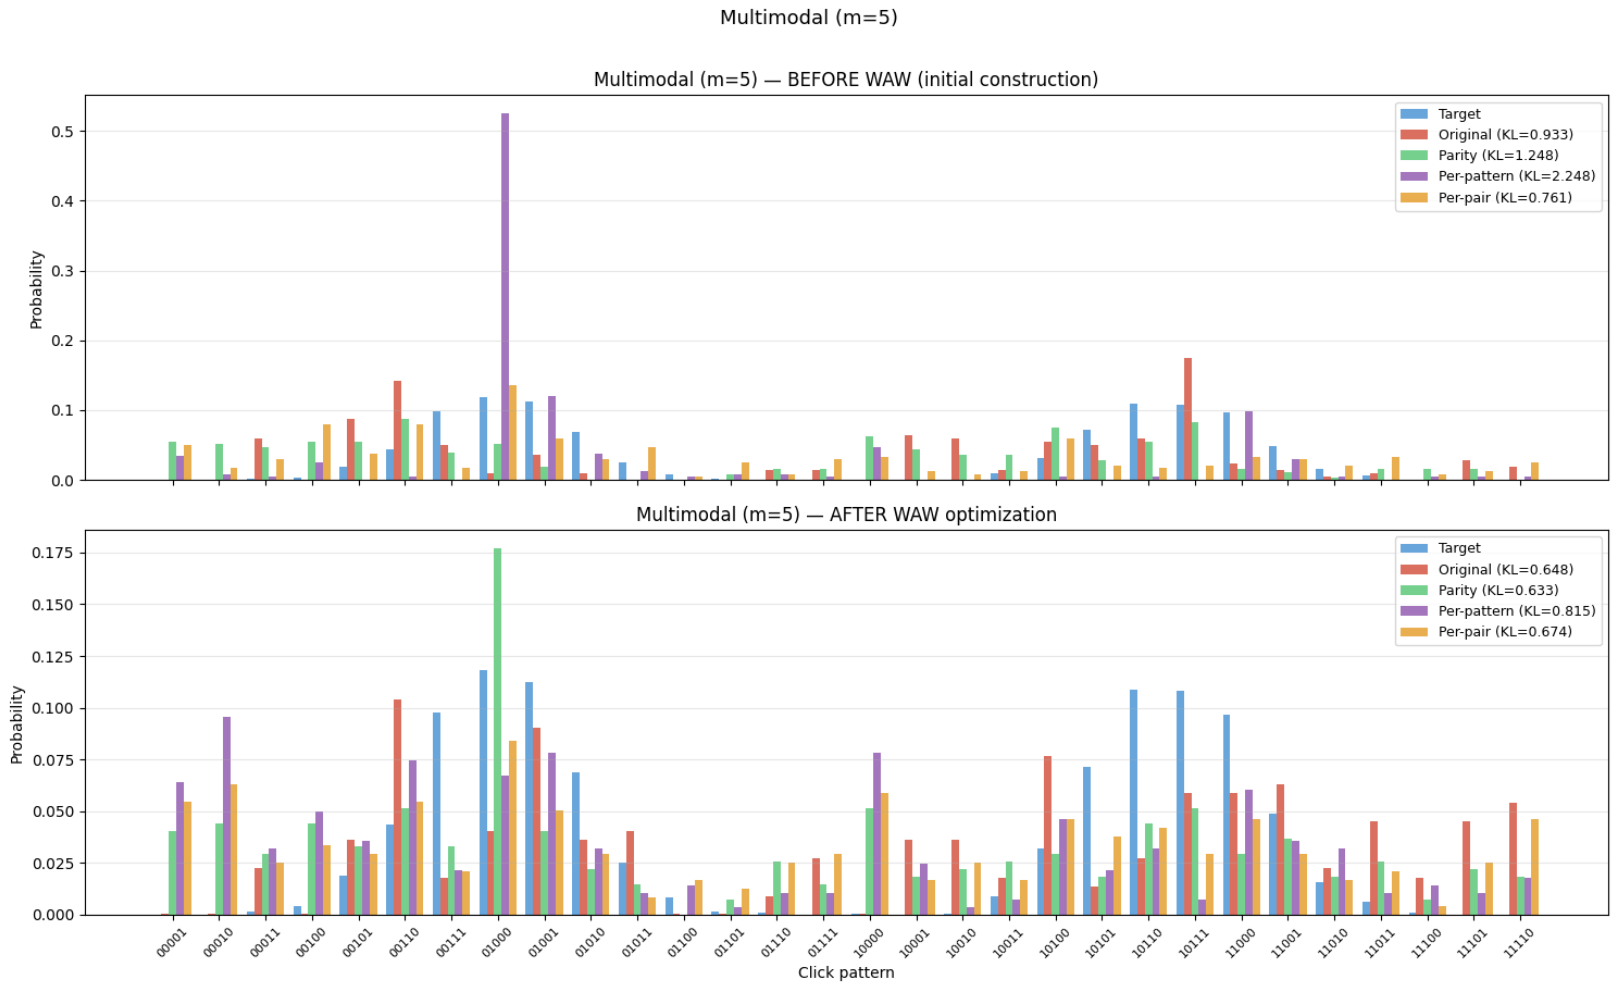
\includegraphics[width=\textwidth]{multimodal_fix.png}
\caption{Multimodal}
\end{subfigure}\hfill
\begin{subfigure}{0.49\textwidth}
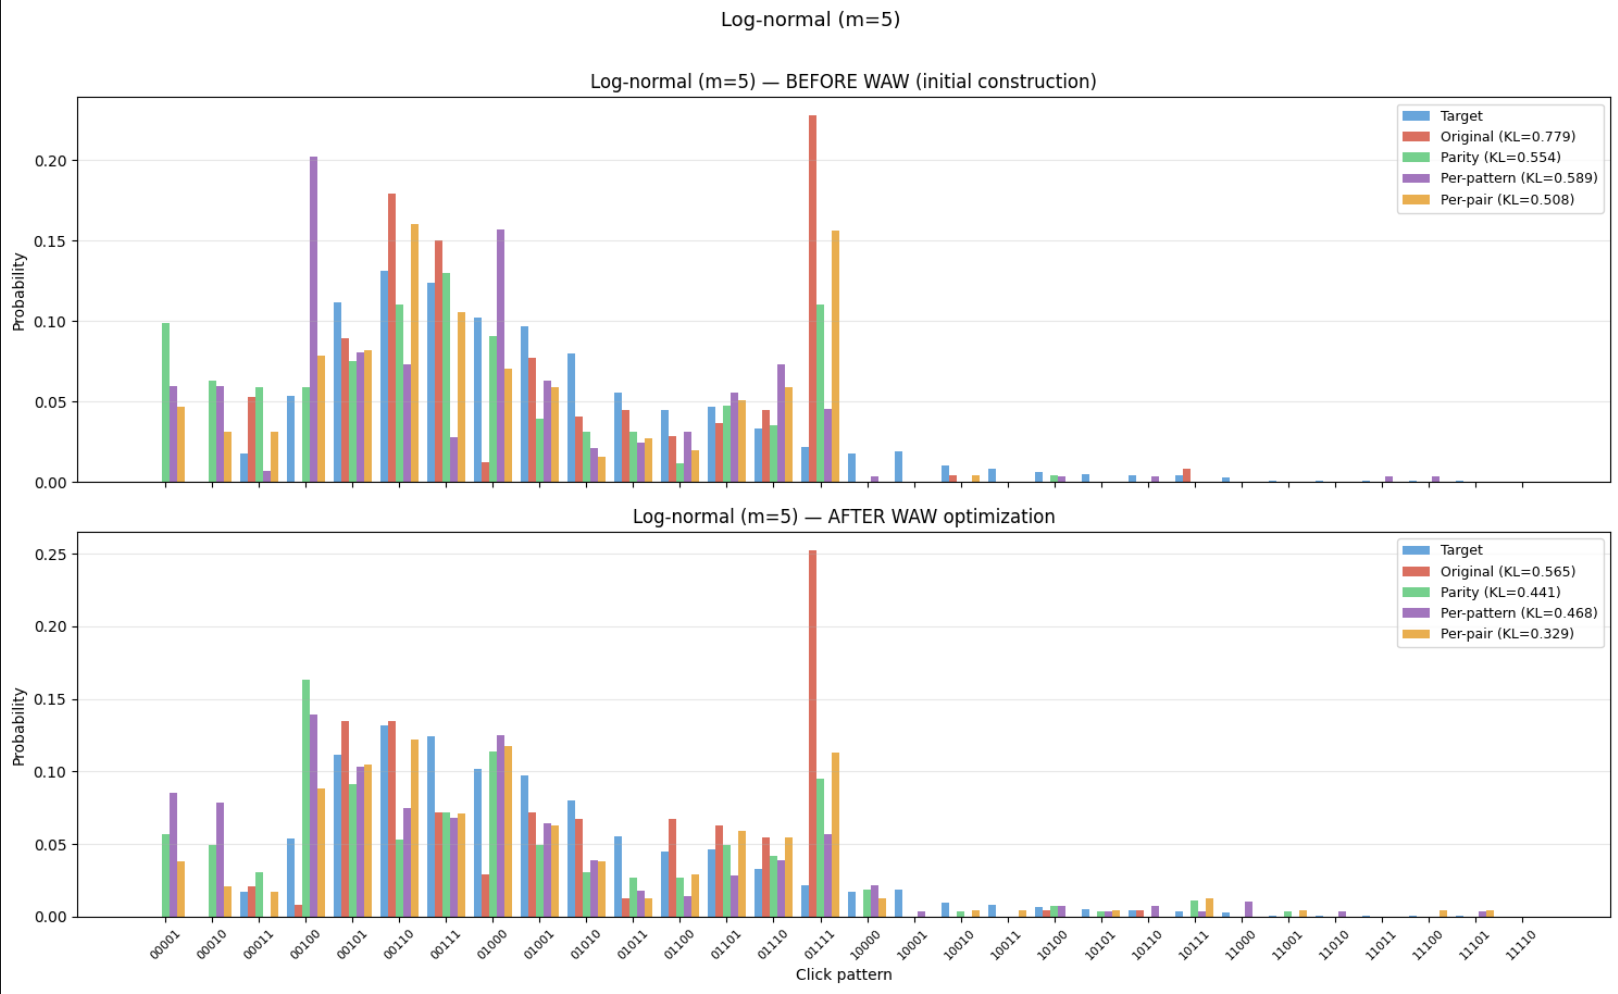
\includegraphics[width=\textwidth]{lognormal_fix.png}
\caption{Log-normal}
\end{subfigure}
\caption{Per-pair construction (green) versus baseline (red) and per-pattern
(purple), before and after WAW.}
\label{fig:fix}
\end{figure}

Figure~\ref{fig:gray} contrasts binary and Gray encoding for the multimodal and
log-normal targets. Under Gray coding the target becomes piecewise-smooth in
pattern order and the two modes of the multimodal target are recovered.

\begin{figure}[h]
\centering
\begin{subfigure}{0.49\textwidth}
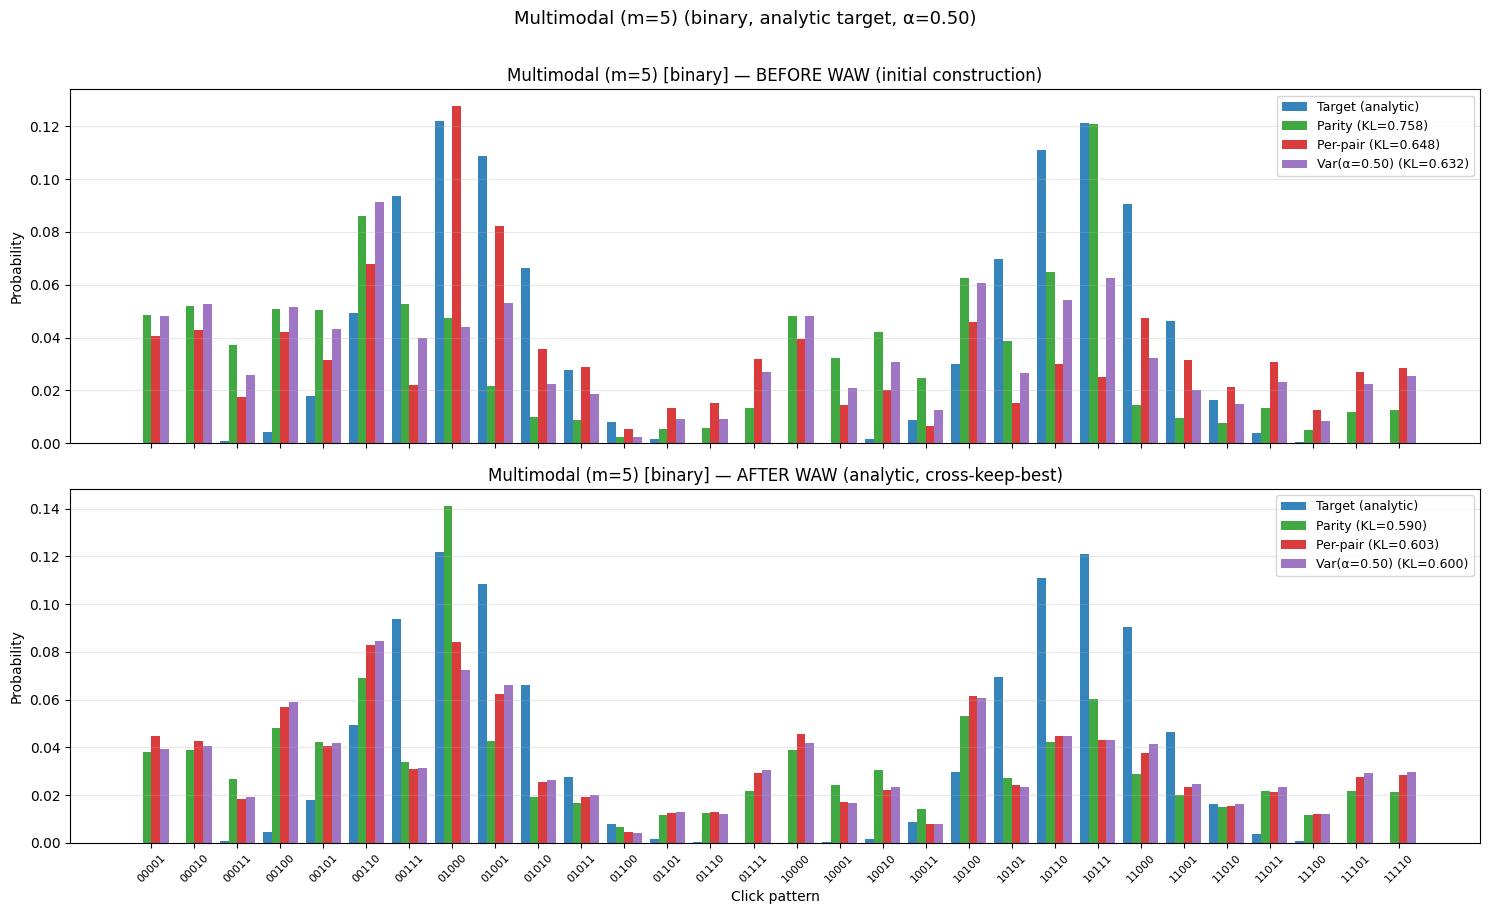
\includegraphics[width=\textwidth]{mmodal_bin.png}
\caption{Multimodal, binary}
\end{subfigure}\hfill
\begin{subfigure}{0.49\textwidth}
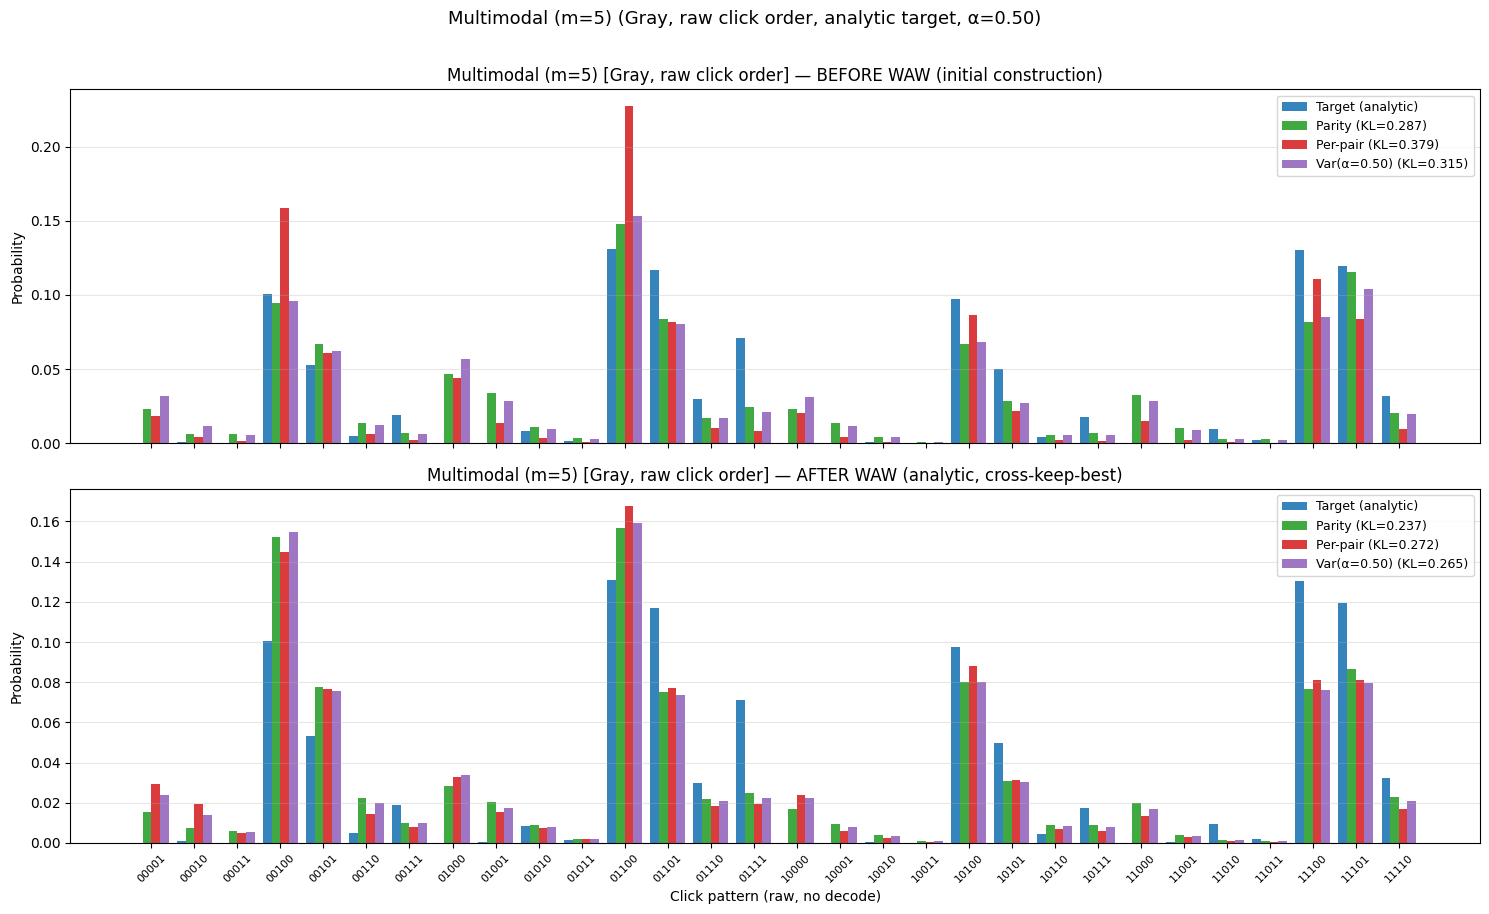
\includegraphics[width=\textwidth]{mmodal_gray.png}
\caption{Multimodal, Gray}
\end{subfigure}

\vspace{4pt}
\begin{subfigure}{0.49\textwidth}
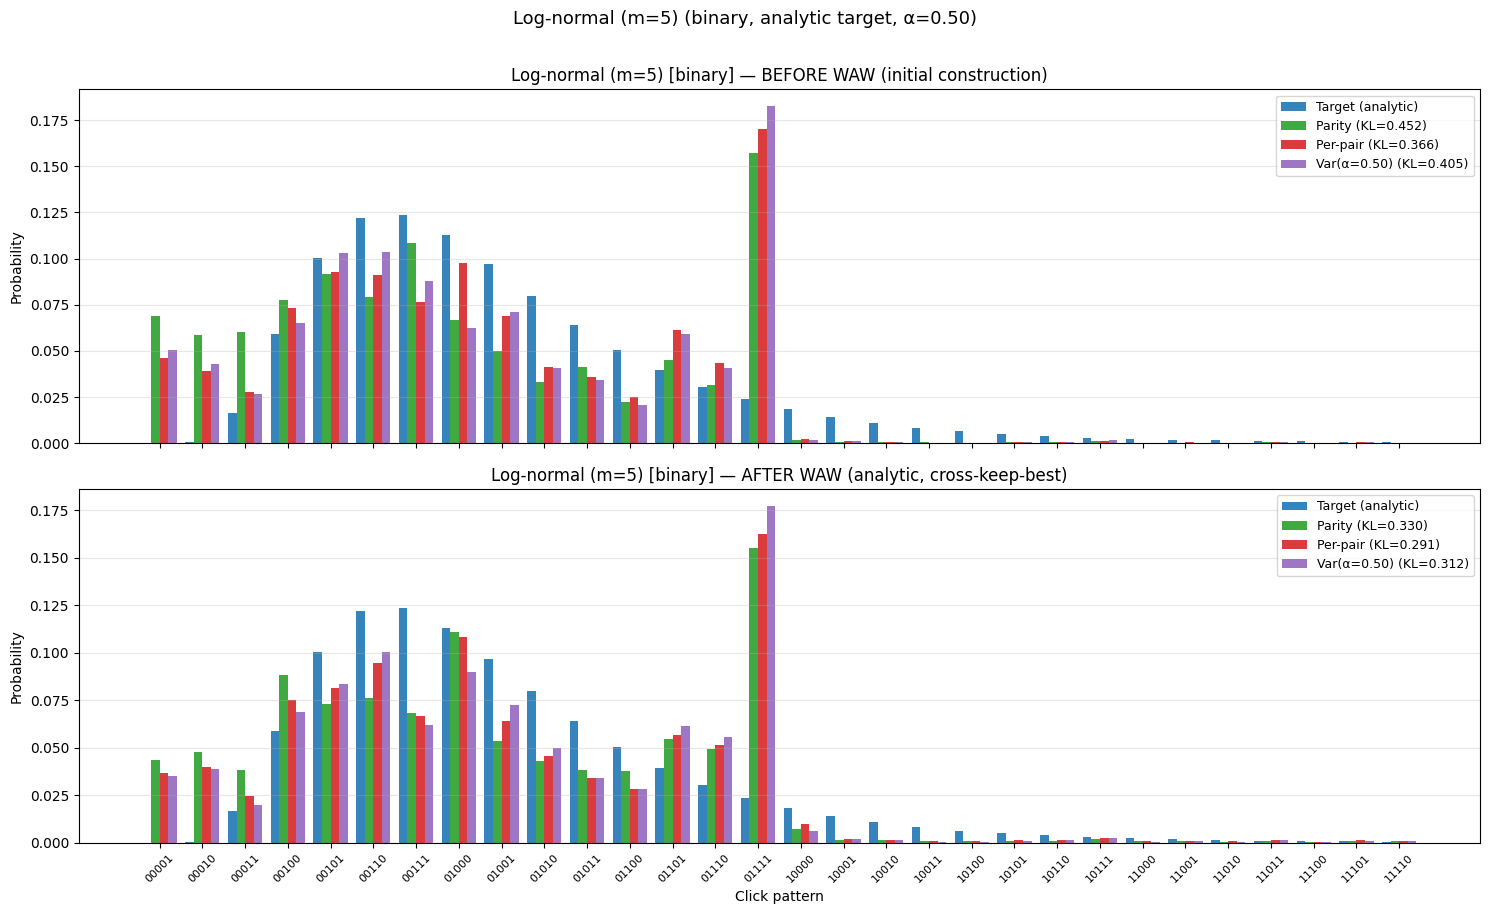
\includegraphics[width=\textwidth]{lognormal_bin.png}
\caption{Log-normal, binary}
\end{subfigure}\hfill
\begin{subfigure}{0.49\textwidth}
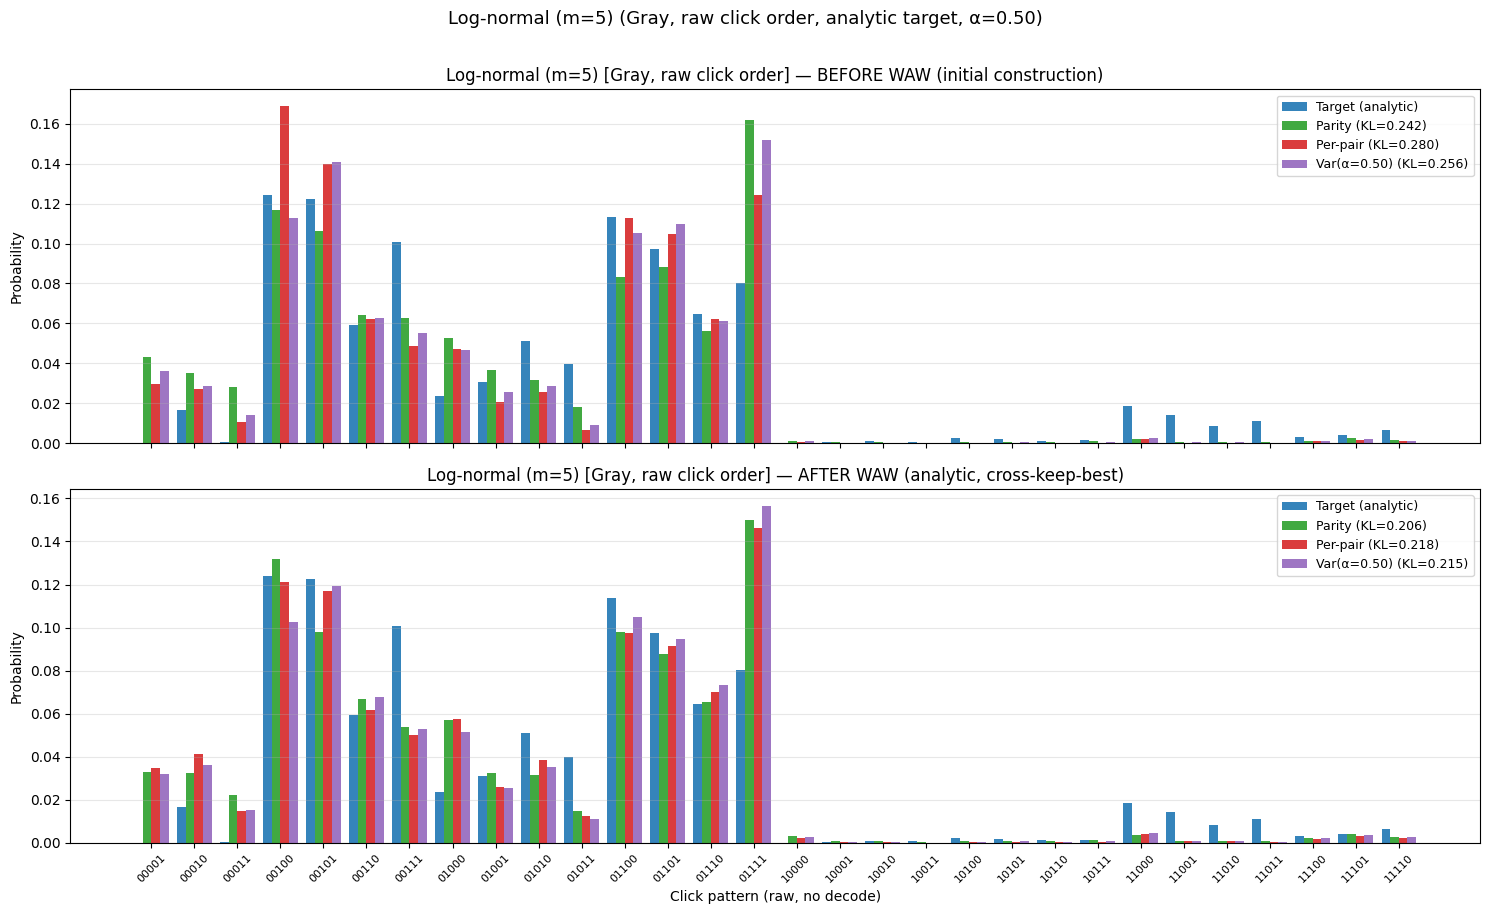
\includegraphics[width=\textwidth]{lognormal_gray.png}
\caption{Log-normal, Gray}
\end{subfigure}
\caption{Standard-binary versus Gray encoding. The effect is largest for the
multimodal target, whose two peaks are shredded across Hamming space under
binary coding.}
\label{fig:gray}
\end{figure}

\subsection{Photon-number matching and reliable optimisation}
Adding the variance construction and the analytic keep-best optimiser removes
two failure modes visible in early runs: the collapse of Gray-encoded WAW onto a
single mode, and the reported KL \emph{increasing} after optimisation (an
artefact of the silent rescale at sampling time). Figure~\ref{fig:var} shows the
combined pipeline (parity/per-pair/variance construction + Gray + keep-best WAW)
for the normal and multimodal targets, displayed in original-bin order so the
target shape is recognisable.

\begin{figure}[h]
\centering
\begin{subfigure}{0.49\textwidth}
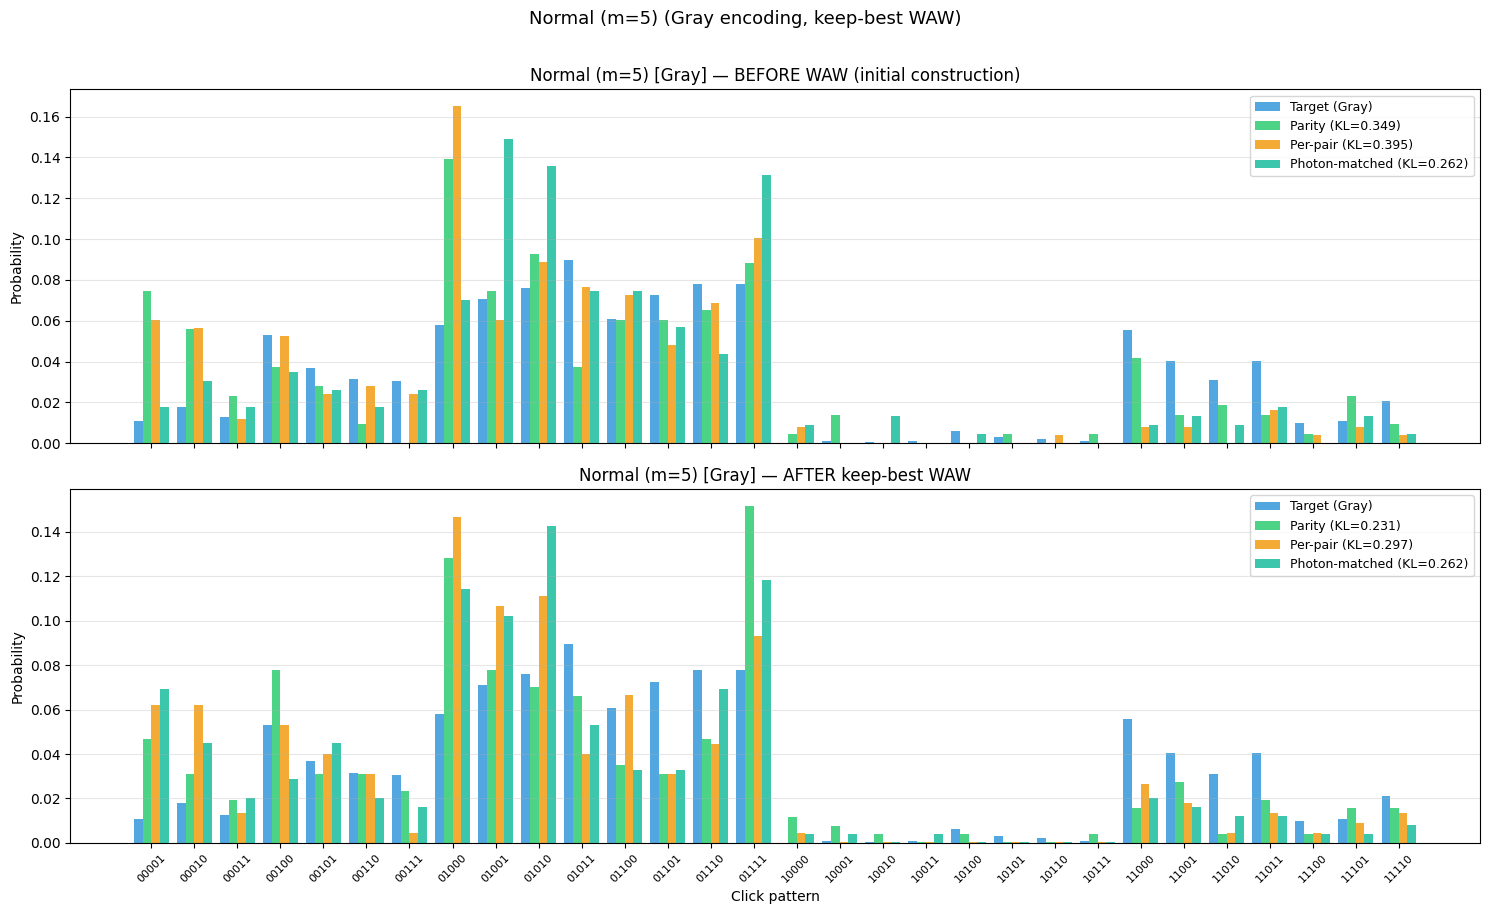
\includegraphics[width=\textwidth]{gray_var_normal.png}
\caption{Normal}
\end{subfigure}\hfill
\begin{subfigure}{0.49\textwidth}
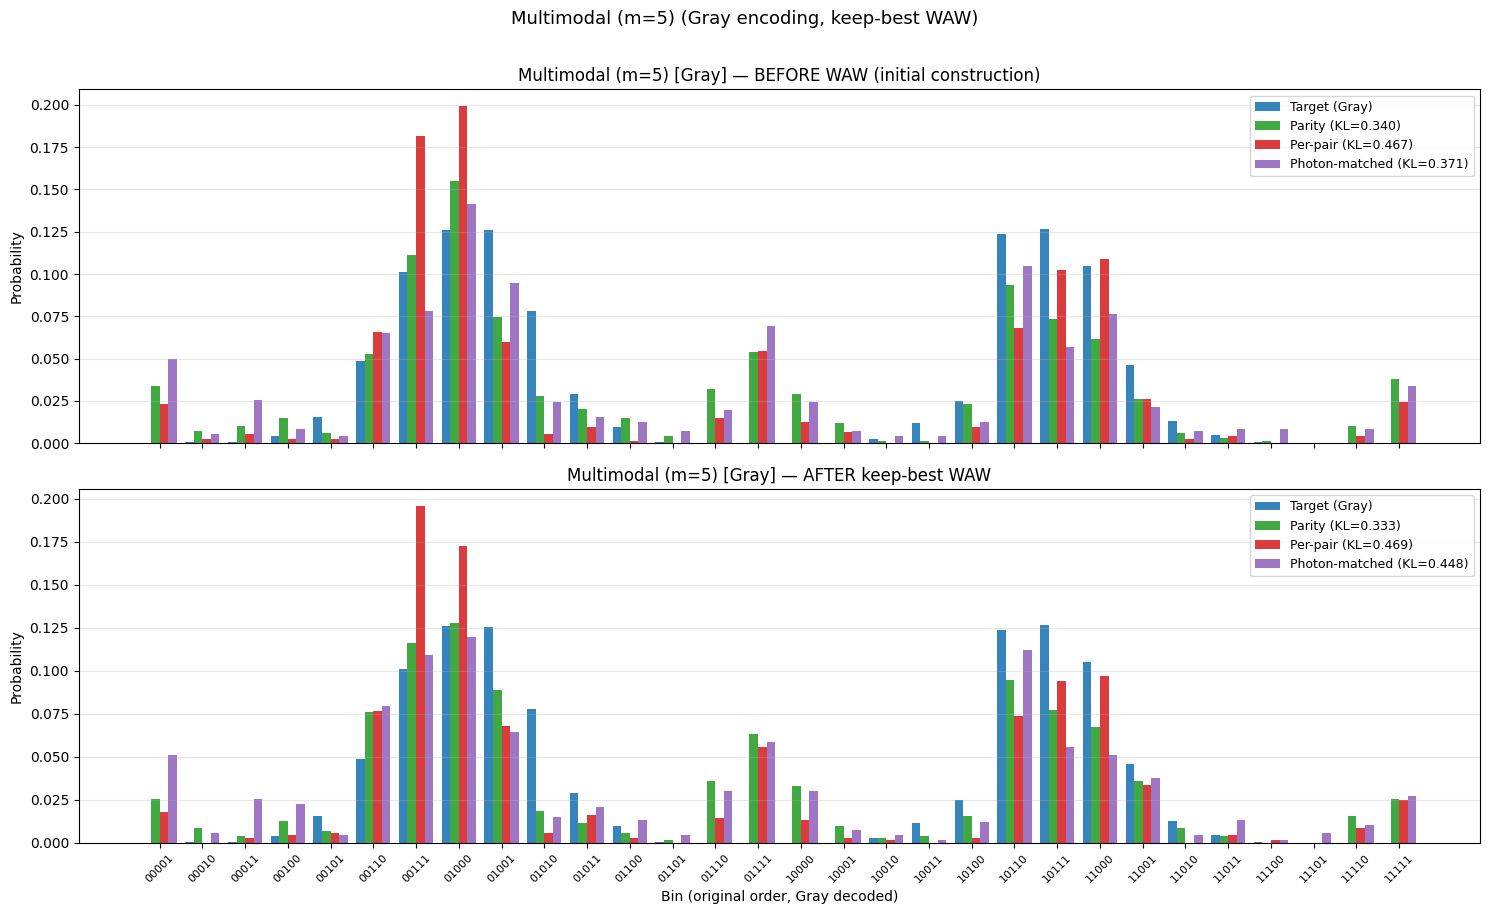
\includegraphics[width=\textwidth]{gray_var_multi_regular.png}
\caption{Multimodal}
\end{subfigure}
\caption{Gray encoding + variance-aware construction + keep-best WAW. The
multimodal panel still shows a residual central bump between the two modes ---
an expressivity floor discussed in Sec.~\ref{sec:concentration}.}
\label{fig:var}
\end{figure}

\subsection{Threshold versus photon-counting readout}
\label{sec:pnr}
Marginalising the exact PNR distribution reproduces the threshold distribution
and quantifies the discarded mass: at $m=4$, ${\sim}20$--$30\%$ of the
probability sits in collision patterns ($n_i\ge 2$) that threshold detection
folds into clicks. Figure~\ref{fig:pnr} compares threshold and full-PNR learning
and opens each threshold click into the photon configurations a counting
detector resolves; the high-photon configurations are probability-starved.

\begin{figure}[h]
\centering
\begin{subfigure}{0.49\textwidth}
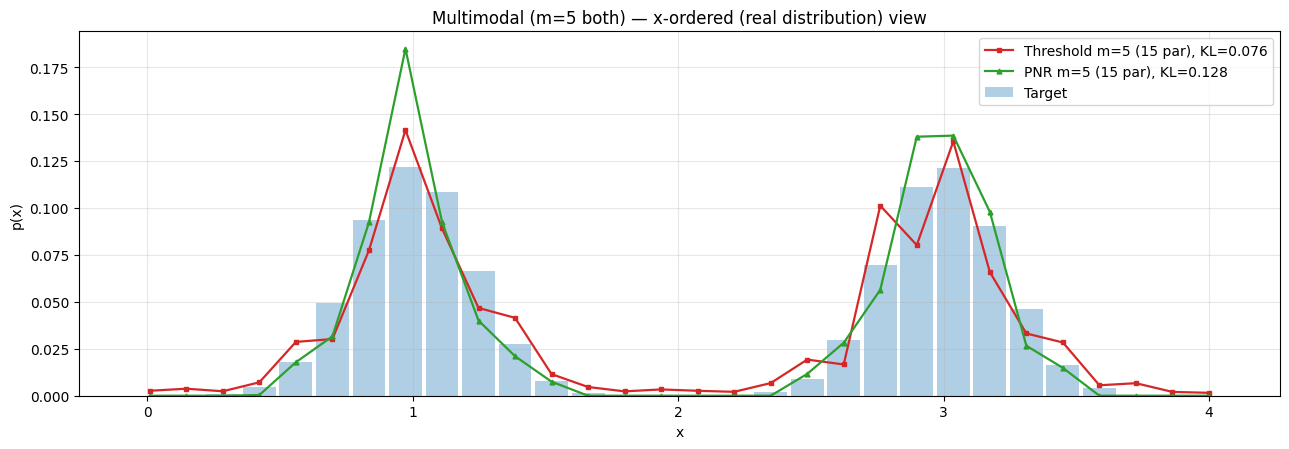
\includegraphics[width=\textwidth]{pnr_mmodal.png}
\caption{Threshold vs PNR (multimodal)}
\end{subfigure}\hfill
\begin{subfigure}{0.49\textwidth}
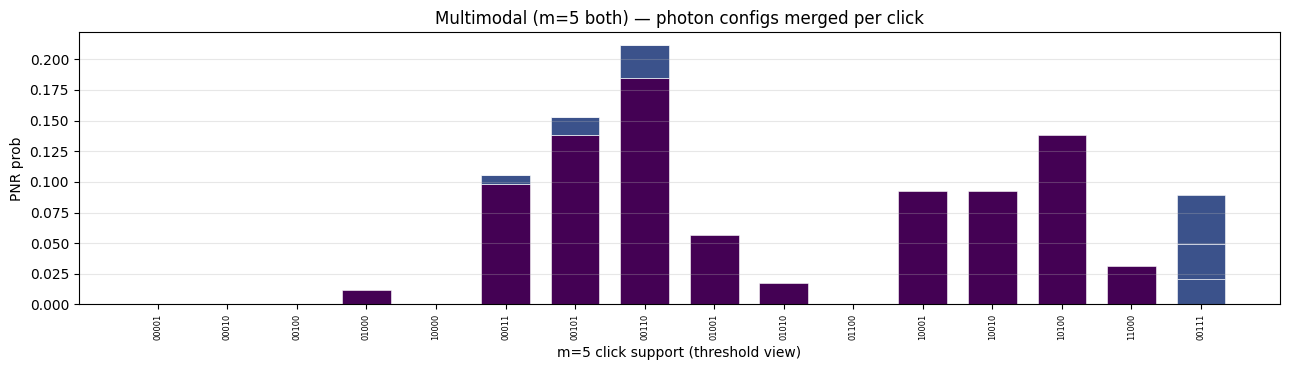
\includegraphics[width=\textwidth]{pnr_merged_mmodal.png}
\caption{PNR configs merged into each click}
\end{subfigure}
\caption{Photon-counting readout. Right: patterns such as $200,400,\dots$ all
read as one threshold click; the stacked mass is dominated by a few low-photon
configurations.}
\label{fig:pnr}
\end{figure}

At fixed modes PNR adds no matrix parameters, and under a probability-matched
encoding it does \emph{not} generally beat threshold learning: its usable
outcomes are dominated by a steep photon-number magnitude hierarchy. The naive
photon-ordered encoding gives a catastrophic $\mathrm{KL}\approx3.7$; a
probability-matched encoding (\texttt{rank\_assign}) is essential.

\subsection{Detector choice matches target concentration}
\label{sec:concentration}
The threshold and PNR model families differ in how concentrated they are. Fitted
at $m=6$, the threshold family is comparatively spread (entropy $3.6$, top-5
pattern mass $0.27$) while the PNR family is concentrated (entropy $3.2$, top-5
mass $0.43$). Matching this to the target's own concentration explains which
detector wins (Table~\ref{tab:conc}): threshold wins on the broad normal target
(${\sim}42/62$ effective bins occupied), PNR wins on the concentrated
asymmetric-bimodal target (${\sim}26/62$ occupied), robustly across 5 seeds.

\begin{table}[h]
\centering
\begin{tabular}{lcc}
\toprule
$m=6$ & Threshold & PNR\\
\midrule
Fitted-model entropy        & 3.6 & 3.2\\
Top-5 pattern mass          & 0.27 & 0.43\\
\midrule
KL, Normal (broad, 42/62)          & \textbf{0.05} & 0.53\\
KL, Asym-bimodal (concentrated, 26/62) & 0.12 & \textbf{0.08}\\
\bottomrule
\end{tabular}
\caption{The concentrated PNR family suits sharply-peaked targets; the spread
threshold family suits broad ones.}
\label{tab:conc}
\end{table}

\subsection{A central spike and its suppression}
\label{sec:spike}
On smooth unimodal targets the learned distribution shows a spike at the peak
bin, ${\approx}2\times$ its neighbours at $m=5$ and ${\approx}2.8\times$ at
$m=6$ (both robust over seeds). It is not a histogram artefact (the empirical
histogram is smooth at the peak, ${\sim}1.1\times$ its neighbours); it is the
model's single most-probable pattern ($q_0/q_1\approx2.3$) mapped onto the peak
bin, which forward KL is content to overshoot. Reverse-KL regularisation does
\emph{not} help --- the concentration is structural for the low-parameter weight
family. The effective control is the mean photon number: the default
$n_{\mathrm{mean}}=m/2$ over-squeezes, and lowering it flattens the head, removes
the spike, and even lowers the KL on broad targets (Table~\ref{tab:spike}). Part
of why the spike is worse at $m=6$ is simply that the default
$n_{\mathrm{mean}}=m/2$ is larger there.

\begin{table}[h]
\centering
\begin{tabular}{lccc}
\toprule
$n_{\mathrm{mean}}$ (Normal, $m{=}6$) & spike/neighbour & $q_0/q_1$ & KL\\
\midrule
1.0            & 1.2 & 1.03 & 0.102\\
\textbf{2.0}   & \textbf{1.5} & \textbf{1.22} & \textbf{0.042}\\
3.0 (default $m/2$) & 2.5 & 2.25 & 0.048\\
4.5            & 4.6 & 3.83 & 0.083\\
9.0            & 6.4 & 5.43 & 0.167\\
\bottomrule
\end{tabular}
\caption{Lowering the mean photon number suppresses the central spike and, near
$n_{\mathrm{mean}}\approx2$, also minimises the KL. Larger values re-inflate it.}
\label{tab:spike}
\end{table}

\subsection{Choosing the mean photon number}
\label{sec:selectnmean}
Since $n_{\mathrm{mean}}=0$ is degenerate (vacuum: no clicks) and a broad target
starved of high-click patterns fits poorly at very small $n_{\mathrm{mean}}$,
there is a target-dependent optimum. It is selected honestly by sweeping
$n_{\mathrm{mean}}$ and minimising the KL to the \emph{empirical} target
(samples only); the choice generalises to the true target (the empirical and
true KL curves coincide). Figure~\ref{fig:nmean} shows the two competing
effects: the fit quality (left) has a minimum whose location depends on the
target, while the central spike (right) grows monotonically with
$n_{\mathrm{mean}}$. The optimum tracks the target's concentration
(Table~\ref{tab:nmean}): broad targets prefer $n_{\mathrm{mean}}\approx2$ ---
already below the default $m/2$ --- while sharply concentrated targets prefer
$n_{\mathrm{mean}}\approx0.5$. In every case the default $m/2$ is suboptimal, so
$n_{\mathrm{mean}}$ should be selected, not hard-wired (\texttt{select\_nmean}).

\begin{figure}[h]
\centering
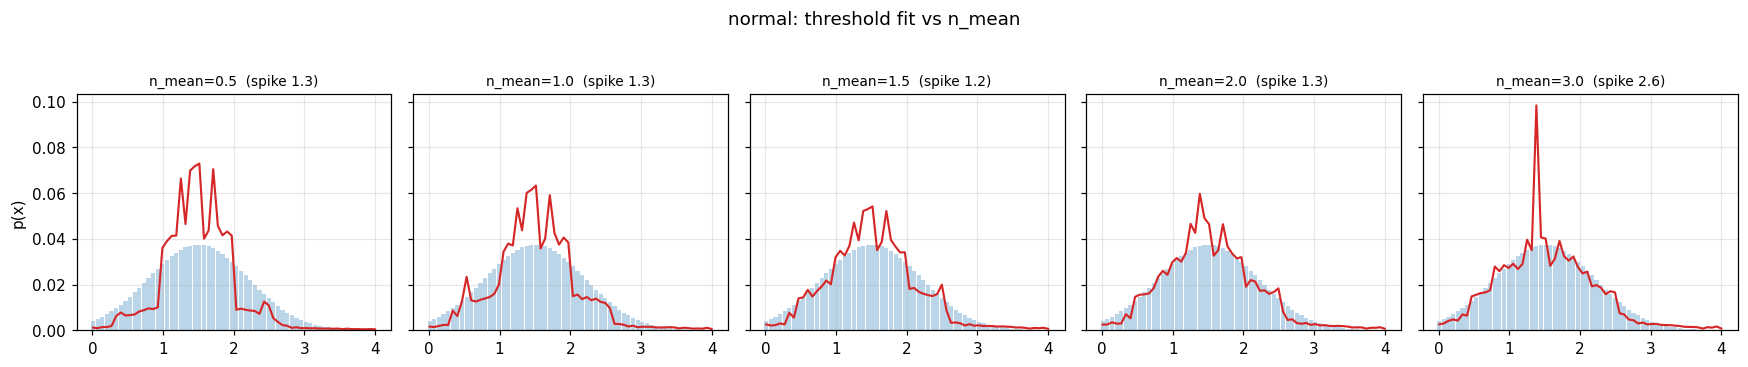
\includegraphics[width=\textwidth]{nmean_sweep_normal.png}
\caption{Normal target ($m=6$): the fitted threshold distribution at
increasing $n_{\mathrm{mean}}$. The central spike (its ratio to the neighbours
is annotated) grows with $n_{\mathrm{mean}}$; too small a value under-fits the
broad body. The best trade-off is around $n_{\mathrm{mean}}=2$.}
\label{fig:nmeangrid}
\end{figure}

\begin{figure}[h]
\centering
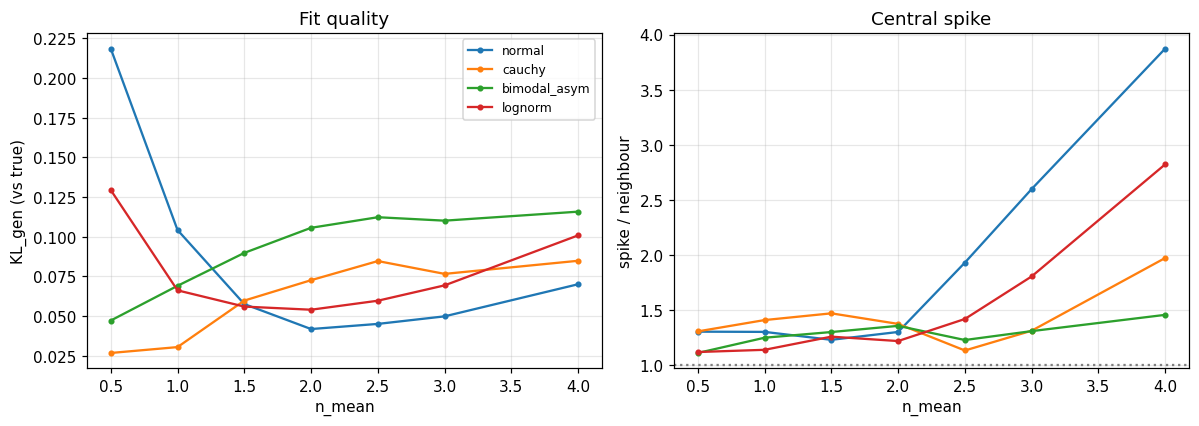
\includegraphics[width=0.86\textwidth]{nmean_selection.png}
\caption{Effect of $n_{\mathrm{mean}}$ across targets ($m=6$). Left: KL to the
true target, with a target-dependent minimum. Right: the central spike grows
monotonically with $n_{\mathrm{mean}}$. Broad targets (normal, log-normal)
optimise near $2$; concentrated targets (Cauchy, asymmetric bimodal) near
$0.5$.}
\label{fig:nmean}
\end{figure}

\begin{table}[h]
\centering
\begin{tabular}{llcc}
\toprule
Target & character & best $n_{\mathrm{mean}}$ & KL$_{\mathrm{gen}}$\\
\midrule
Normal        & broad         & 2.0 & 0.042\\
Log-normal    & moderate      & 2.0 & 0.054\\
Cauchy        & sharp peak    & 0.5 & 0.027\\
Asym.\ bimodal & concentrated  & 0.5 & 0.047\\
\bottomrule
\end{tabular}
\caption{Selected $n_{\mathrm{mean}}$ (by minimum empirical KL, $m=6$). The
optimum decreases with the target's concentration; all are below the default
$m/2=3$.}
\label{tab:nmean}
\end{table}

\subsection{Outlier suppression and its limits}
Forward KL is zero-avoiding: where the target is ${\sim}0$ (a valley), it does
not penalise stray model mass, so valley outliers (e.g.\ the \texttt{10000} bump
in the multimodal gap) survive. A reverse-KL term (\texttt{train\_WAW\_mixed})
penalises exactly $q>p$ overshoot, but on the multimodal target the valley mass
falls only from $0.386$ to $0.367$ as $\beta$ grows from $0$ to $0.6$ while the
forward KL rises. The weak response is itself informative: those outliers are
structural (a single Gaussian state is forced to emit inter-mode mass), not an
objective artefact. Reverse KL cleanly removes only \emph{removable} outliers.

\subsection{Honest evaluation: encoding estimated from samples}
The probability-matched encoding must not peek at the true target. Using the
\emph{empirical} histogram $\hat p$ (from samples only) for both the encoding and
the training objective, and the true target only to report a generalisation KL,
gives KL$_{\mathrm{train}}\approx$ KL$_{\mathrm{gen}}$ (no overfitting of
sampling noise). Table~\ref{tab:oracle} shows the empirical encoding matches the
oracle and both far outperform the fixed integer encoding --- the small oracle
advantage is not a hidden cheat but a robust property of the encoding. A
sample-size sweep indicates ${\sim}50$--$100$ samples per bin suffice before the
model's expressivity floor dominates.

\begin{table}[h]
\centering
\begin{tabular}{lc}
\toprule
Threshold $m{=}5$, Normal & KL\\
\midrule
Standard-binary (integer) encoding & 0.21\\
\texttt{rank\_assign} (oracle, true target) & 0.06\\
\texttt{rank\_assign} (empirical $\hat p$, samples only) & 0.06\\
\bottomrule
\end{tabular}
\caption{The encoding is realizable from samples alone; the oracle is not
cheating.}
\label{tab:oracle}
\end{table}

\section{Combining threshold and photon-counting readouts}
\label{sec:combine}
Sections~\ref{sec:pnr}--\ref{sec:concentration} showed that the threshold and
PNR readouts are complementary: threshold is a spread family (good on broad
targets), PNR a concentrated one (good on sharp peaks). Since both fitted models
can be mapped back to the same $x$-bins (by inverting their probability-matched
encoding), they can be combined there. We use a convex mixture
\begin{equation}
q_{\mathrm{mix}}(x) = w\,q_{\mathrm{thr}}(x) + (1-w)\,q_{\mathrm{PNR}}(x),
\end{equation}
with the weight $w$ chosen by minimising the KL to the \emph{empirical} target
(samples only). This is physically realizable --- run each detector with
probability $w$ per shot --- and, being a convex combination, is never worse
than the better single model. A product-of-experts variant
$q\propto q_{\mathrm{thr}}^{w}q_{\mathrm{PNR}}^{1-w}$ was also tested
(\texttt{combine\_threshold\_pnr}).

Table~\ref{tab:combine} reports the outcome. On pure-broad (normal) and
skewed (log-normal) targets the mixture correctly defaults to (almost) all
threshold ($w^\star\!\to\!1$), matching the better model. On targets with
\emph{mixed} structure it beats both single readouts substantially: the Cauchy
target (a sharp peak on broad tails) drops from $0.083$/$0.615$ to $0.025$ at an
even $w^\star=0.5$ (Fig.~\ref{fig:combine}), and the asymmetric bimodal from
$0.114$/$0.077$ to $0.039$. The mechanism is visible in
Fig.~\ref{fig:combine}: threshold supplies the broad tails that PNR
underproduces, while PNR supplies the sharp peak that threshold overshoots, so
their mixture tracks the target where neither alone can.

\begin{table}[h]
\centering
\begin{tabular}{lcccc}
\toprule
Target ($m{=}6$) & Threshold & PNR & Mixture & $w^\star$\\
\midrule
Normal        & \textbf{0.047} & 0.537 & 0.047 & 1.00\\
Log-normal    & \textbf{0.051} & 0.280 & 0.050 & 0.86\\
Cauchy        & 0.083 & 0.615 & \textbf{0.025} & 0.50\\
Asym.\ bimodal & 0.114 & 0.077 & \textbf{0.039} & 0.14\\
\bottomrule
\end{tabular}
\caption{KL to the true target for the single readouts and their empirical-best
convex mixture. The mixture never loses and wins by $2$--$3\times$ on targets
with both broad and sharp structure.}
\label{tab:combine}
\end{table}

\begin{figure}[h]
\centering
\begin{subfigure}{0.49\textwidth}
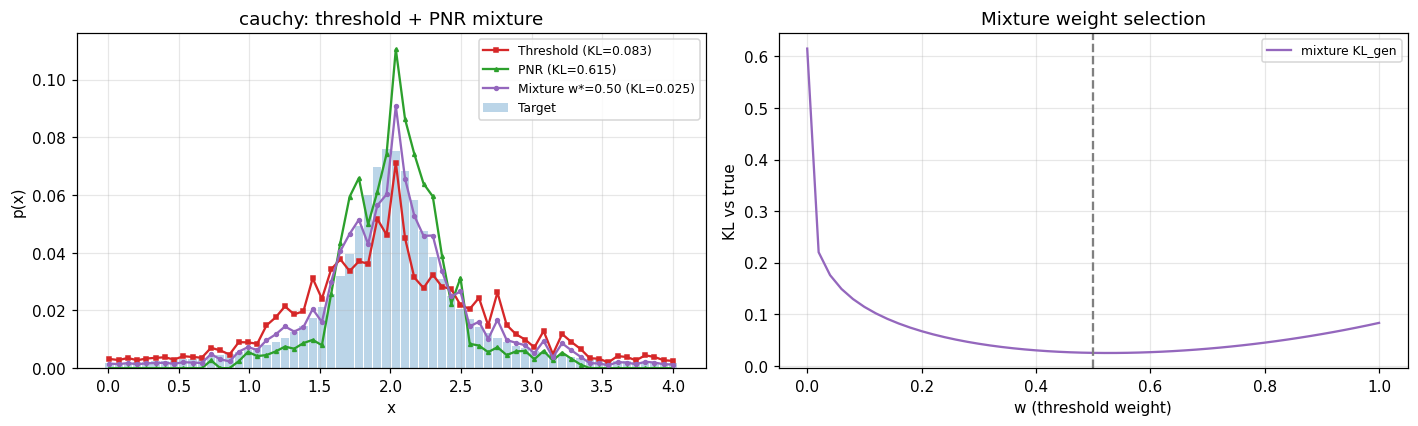
\includegraphics[width=\textwidth]{combine_cauchy.png}
\caption{Cauchy}
\end{subfigure}\hfill
\begin{subfigure}{0.49\textwidth}
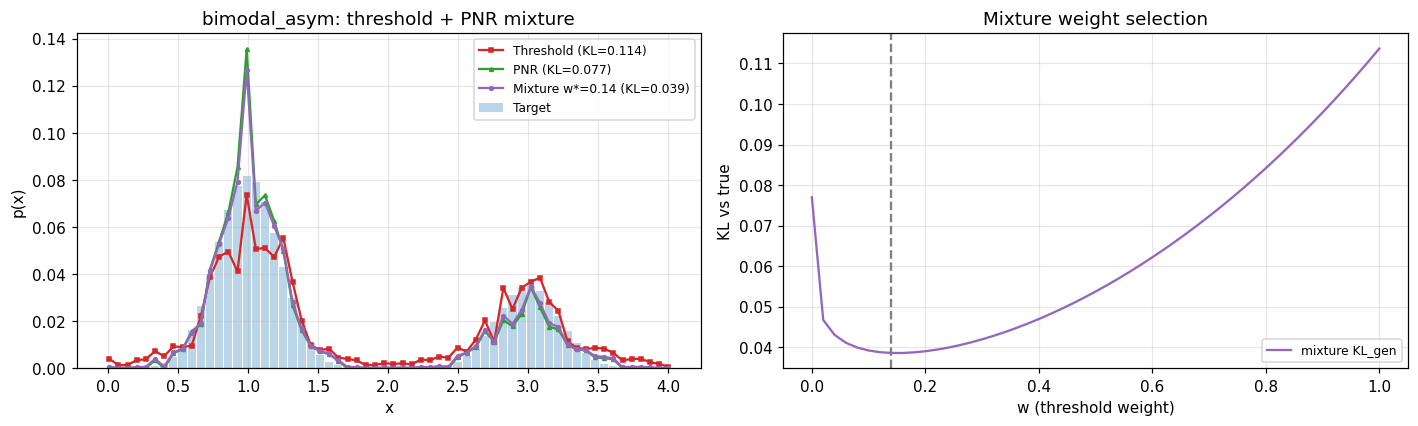
\includegraphics[width=\textwidth]{combine_bimodal_asym.png}
\caption{Asymmetric bimodal}
\end{subfigure}
\caption{Threshold + PNR convex mixture (purple) against the single readouts.
Left panels: distributions; right panels: KL versus mixing weight $w$, with a
clear interior optimum. The mixture beats both single readouts.}
\label{fig:combine}
\end{figure}

\section{Conclusions and outlook}
The GBS distribution-learning pipeline has several orthogonal bottlenecks, each
individually addressable: the initial construction (parity / per-pair /
variance), the encoding (Gray + probability matching), the optimiser (analytic
keep-best), the photon budget (mean via $n_{\mathrm{mean}}$, variance via
click-count matching), and the detector (threshold vs counting). Their
combination reduces the KL by about a factor of three on smooth targets and
$2.5\times$ on the multimodal target.

Two levers introduced here give further gains without new physics. First, the
mean photon number should be \emph{selected} rather than fixed to $m/2$: it
trades the central spike against high-click coverage, and its optimum tracks the
target's concentration (Sec.~\ref{sec:selectnmean}). Second, the threshold and
photon-counting readouts are complementary and their empirical-best convex
mixture never loses and wins by $2$--$3\times$ on targets with both broad and
sharp structure (Sec.~\ref{sec:combine}); the mixture is physically realizable
as a per-shot choice of detector.

Two structural limits remain and are now well characterised: the multimodal
valley is an expressivity floor of a single Gaussian state (neither objective
reweighting nor encoding removes it), and single detectors are concentration-
limited. The natural next step is added expressivity --- displacement (already
prototyped) or a small mixture of GBS states --- evaluated under the honest,
sample-only protocol and the analytic KL used here.

\begin{thebibliography}{9}
\bibitem{banchi2020}
L.~Banchi, N.~Quesada, J.~M.~Arrazola,
\textit{Training Gaussian Boson Sampling Distributions},
Phys.\ Rev.\ A \textbf{102}, 012417 (2020). arXiv:2004.04770.

\bibitem{quesada2018}
N.~Quesada, J.~M.~Arrazola, N.~Killoran,
\textit{Gaussian boson sampling using threshold detectors},
Phys.\ Rev.\ Lett.\ \textbf{121}, 110503 (2018). arXiv:1807.01639.

\bibitem{hamilton2017}
C.~S.~Hamilton \textit{et~al.},
\textit{Gaussian Boson Sampling},
Phys.\ Rev.\ Lett.\ \textbf{119}, 170501 (2017). arXiv:1612.01199.

\bibitem{kruse2019}
R.~Kruse \textit{et~al.},
\textit{Detailed study of Gaussian boson sampling},
Phys.\ Rev.\ A \textbf{100}, 032326 (2019). arXiv:1801.07488.
\end{thebibliography}

\end{document}
